%
% @author Kalvin Döge
%


\section{Stand der Wissenschaft}\label{sec:state-of-science}

Die Idee, Lichtsignalanlagen an Kreuzungen mit einer vorherbestimmten Steuerung zu verwalten, ist aber keine neue.
Mehrere Forscher haben bereits Lösungen über künstliche Intelligenzen, durch Fokussierung auf die Fahrradfahrer oder zeitlicher Abstimmung von den Lichtsignalphasen gefunden.

\textbf{Ye Zheng, Ding Ma, Fengying Jin und Zhigang Zhao:}
\textit{Intelligent Traffic Signal Control Based on Reinforcement Learning with State Reduction for Smart Cities}

In dem Forschungsbeitrag von Li Kuang und andere aus dem Jahr 2019, widmen sich die vier Autoren einer Lösung mithilfe eines Q-Learning-Algorithmus.
Dadurch, dass die Infrastruktur der Straßen nicht weiter ausgebaut werden kann in urbanem Verkehr, bleibt nur noch das Auflösen von Staus bei Lichtsignalschaltung und Kreuzungen\cite{Zheng2019}, weshalb sie sich mit dieser Arbeit an den Ansatz mit einer künstlichen Intelligenz setzten.

Die bisher entwickelten Echtzeitlösungen, so Zheng und andere, lassen sich in vier Kategorien unterordnen:
Feste Zeitschaltungen mit Anpassungen je Tageszeit, vorhersagende Signalschaltungen aufgrund von Eingabedaten aus vergangenem oder aktuellem Verkehrsfluss, Betätigungssignalschaltungen, die bei Aktivierung von Sensoren die Grün- oder Rotphasen verlängern, und die Adaptivschaltung, die mit Sensoren und Algorithmen den Verkehr zum Zeitpunkt des Eintretens die Schaltungen verändern\cite{Zheng2019}.

Der Ansatz ihrer Arbeit mit der künstlichen Intelligenz fällt unter eine neue Lösungsstrategie, mit der sie Lichtsignalphasen bei einzelnen Kreuzungen über das verstärkte Lernen abstimmen wollen\cite{Zheng2019}.
Beispielsweise sind gegenüberliegende, geradlinig gerichtete Straßenspuren, wie in der Grafik~\ref{fig:kuang-lanes} bei zum Beispiel den Spuren 6 und 2 zu sehen ist, miteinander verknüpfbar zu einer Lichtsignalphase, da sie keine überkreuzenden Fahrbahnen besitzen.
Um diese Phaseneinteilung für die künstliche Intelligenz vorzubereiten, sollen die einzelnen Fahrbahnkombination mit den Fahrzeugdaten in Klassen unterteilt werden\cite{Zheng2019}.

\begin{figure}[h]
    \centering
    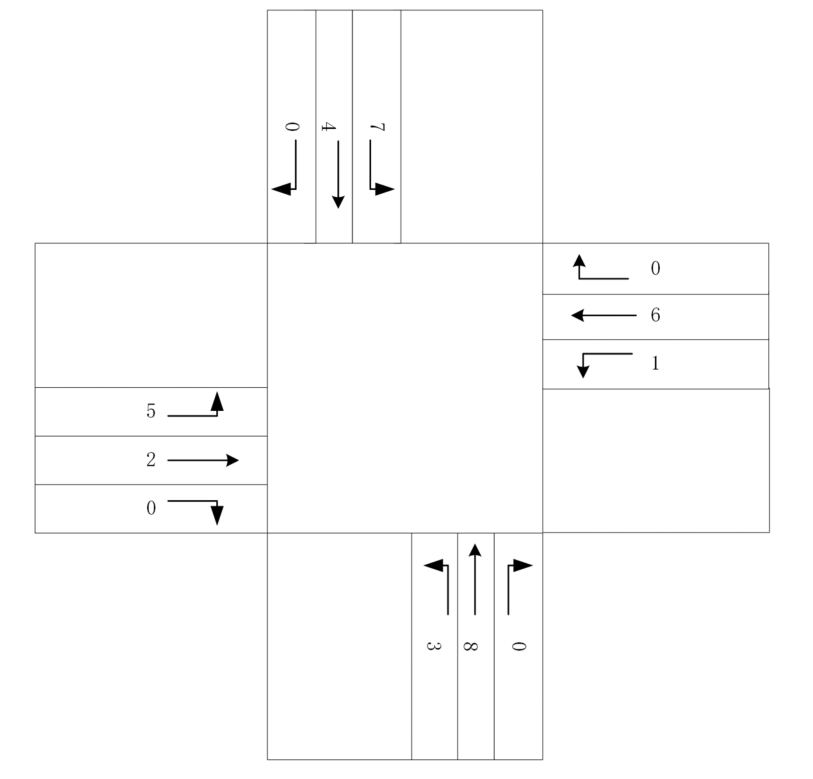
\includegraphics[width=0.75\textwidth]{kuang-lanes}~\caption{Das von Kuang und andere bei einer dreispurigen Kreuzung dargelegte 8-Phasen Modell~\cite{Zheng2019}}
    \label{fig:kuang-lanes}
\end{figure}

Weiter verbessern sie den Algorithmus, indem sie seltene oder fast nie auftretende Szenarien aus der Menge möglicher Zustände entfernen und durch die Kombinierung von Spuren weniger Werte in die Eingabe der künstlichen Intelligenz geben müssen.

Im Folgenden gehen sie auf weitere Arbeiten ein, die eine andere Größenskalierungen als sie vorgenommen haben, bevor sie dann auf die genaue Implementation des Straßenmodells und dem Lernen beziehungsweise Trainieren der künstlichen Intelligenz selbst eingehen.

Ein Problem bei ihrer Phaseneinteilung ist aber, dass sie bei Kreuzungen je drei eingehende Spuren annahmen.
Auch wenn die Stauzonen meist große Kreuzungen sind, so haben Städte auch Lichtsignalschaltungen an verschiedene Kreuzungen mit mehr als nur drei oder auch zwei Spuren, sodass ein Q-Learning-Algorithmus nicht mit solchen Szenarien umgehen kann und bei anderen Kreuzungen neukonzipiert und trainiert werden muss.

Dennoch ist die Einteilung der verschiedenen Lösungsansätze ein wichtiger Aspekt, der auch in dieser Arbeit Relevanz hat, explizit der erste Typ, die feststehende Zeitschaltung.


\textbf{Valentina Kurtc und Martin Treiber:}
\textit{Simulating bicycle traffic by the intelligent-driver model-Reproducing the traffic-wave characteristics observed in a bicycle-following experiment}

Der Forschungsbeitrag von Kurtc und Treiber aus dem Jahr 2020 untersucht die Hypothese, dass sich die Bewegungsdynamik des Fahrzeugverkehrs qualitativ nicht unterscheidet von dem Fahrradverkehr, indem sie die Qualität eines Fahrzeugmodells beziehungsweise Pkw-Modells ebenso für Fahrräder nutzen können.
Dies beweisen sie mit einem ,,Intelligent Driver Model``\cite{Kurtc2020}, einem mikroskopischen Modell für Autos, und vergleichen dessen Qualität der Kalibrierung und Vorhersagefähigkeit dann mit dem ,,Necessary Decelaration Model``\cite{Kurtc2020}, einem mikroskopischen Fahrradmodell.

Im Folgenden gehen Kurtc und andere darauf ein, wie sie eine Vergleichsbasis über die Formel herstellen und das anhand der Beschleunigungsfunktionen aus den Modellen aufbauen, um dann ein Kreisverkehrsszenario mit einem Fahrraddatenset zu simulieren und die berechneten Ergebnisse zu vergleichen.

\begin{figure}[h]
    \centering
    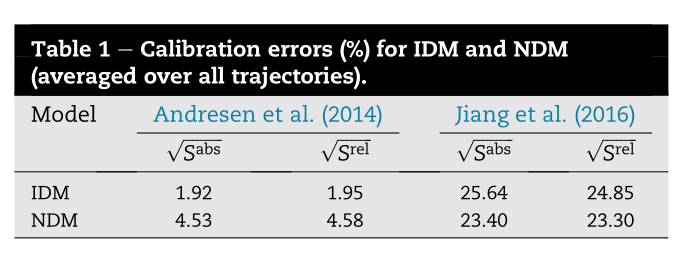
\includegraphics[width=0.75\textwidth]{kurtc2020}~\caption{die von Kurtc und Treiber berechneten, durchschnittlichen Kalbirierungsfehler der beiden Modelle in \%~\cite{Kurtc2020}}
    \label{fig:kurtc2020}
\end{figure}

Das Ergebnis aus der Grafik~\ref{fig:kurtc2020} zeigt, dass die Unterschiede der Modelle beim Nutzen von Fahrraddaten klein sind, als dass sie keinen großen Effekt auf die Simulationen haben.

Aus Kurtc und Treibers Forschungsarbeit lässt sich für diese Simulation also ableiten, dass Agenten, die auf der Straße fahren und Modalitäten wechseln, sowohl mit den Bewegungsmodellen von Fahrrad und Auto simuliert werden können, ohne an Akkuratheit einbüßen zu müssen.


\textbf{Saif Islam Bouderba und Najem Moussa:}
\textit{Reinforcement Learning (Q-LEARNING) traffic light controller within intersection traffic system}

In dem Thesenpapier von Bouderba und Moussa aus dem Jahr 2020 wird eine ähnliche Hypothese wie die von Kuang und andere untersucht.
Sie untersuchen die Effektivität von drei Lösungsansätzen für ihr zelluläres Automatenmodell:
Bei dem ersten Experiment simulieren sie einen einfachen, synchronisierten Ablauf der Lichtsignalschaltungen, beim Zweiten einen Ansatz einer ,,Grünen Welle``-Schaltung mit aufeinanderfolgenden Ampeln und beim Dritten eine durch Q-Learning-Algorithmus gesteuerte Kreuzung~\cite{Bouderba2019}.

Ihr Automatenmodel besteht dabei aus einer Matrix an Kreuzungen, die alle von der Position her mit ihren umliegenden Nachbarn über eine zweispurige Straße verbunden sind:

\[N \times N = 4\]

Jede Kreuzung hat also vier Eingangs- und Ausgangspunkte sowie eine Lichtsignalanlage, die mit je einer Lösungsstrategie pro Experiment gesteuert wird.
Zudem ist die Simulationsumgebung aufgeteilt in Zellen, auf denen sich die Agenten entlangbewegen und zu den Kreuzungen gelangen\cite{Bouderba2019}.

\begin{figure}[h]
    \centering
    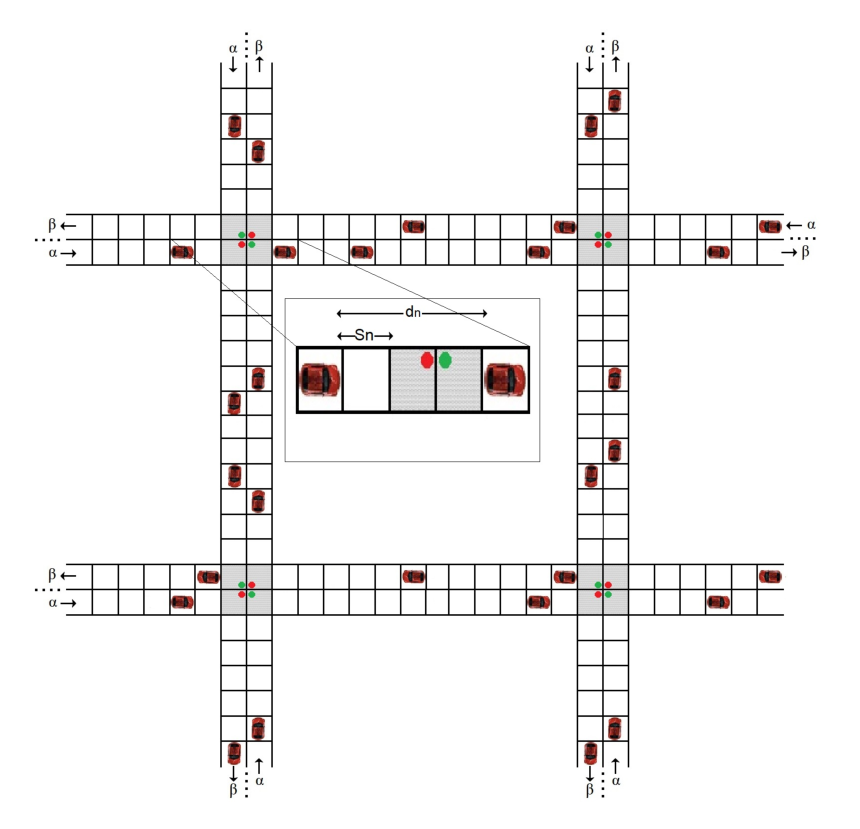
\includegraphics[width=0.75\textwidth]{bouderba-cells-model}~\caption{Eine Momentaufnahme aus dem zellulären Automatenmodell~\cite{Bouderba2019}}
    \label{fig:bouderba-cells-model}
\end{figure}

Mit dem Modell~\ref{fig:bouderba-cells-model} als Simulationsgrundlage erläutern Bouderba und Moussa ihre vorgestellten Lösungsstrategien.
Die grüne Welle Synchronisation erfolgt über eine Verschiebung der aktuellen, internen Zeituhr von umliegenden Lichtsignalen, während der Q-Learning-Alhorithmus trainiert wird, um eine passende Schaltung selbst zu erlernen.

\begin{figure}[h]
    \centering
    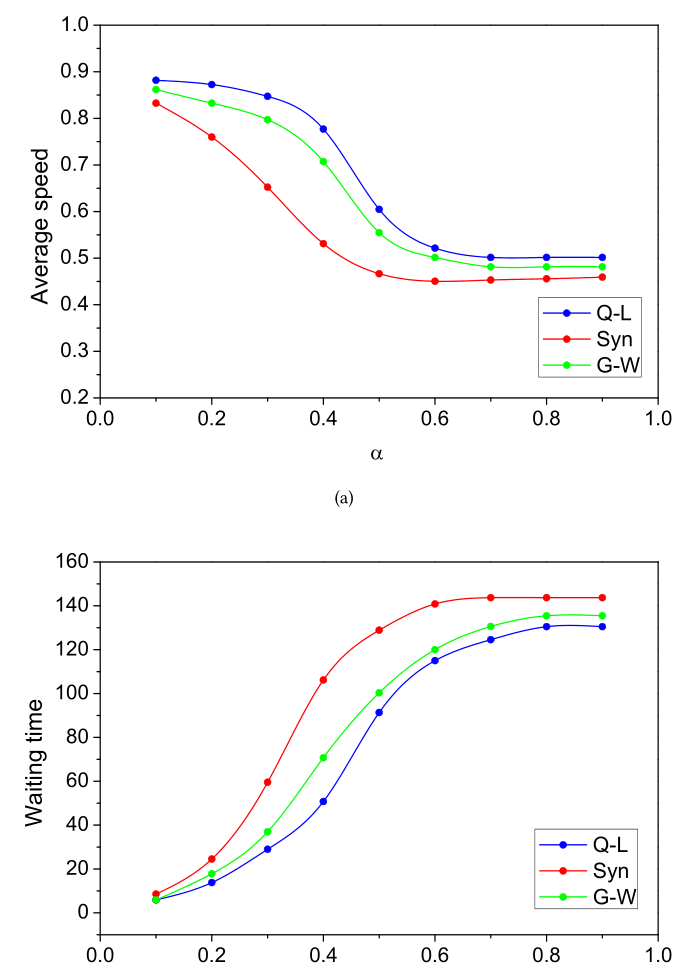
\includegraphics[width=0.5\textwidth]{bouderba-results}~\caption{Die durchschnittliche Geschwindigkeit und Wartezeit nach Durchführunge~\cite{Bouderba2019}}
    \label{fig:bouderba-result-graph}
\end{figure}


Die Resultate aus Grafik~\ref{fig:bouderba-result-graph}, die in Geschwindigkeit und Wartezeit pro Eingriffsrate dargestellt sind, zeigen auf, dass der einfache, synchronisierte Ansatz am schlechtesten von allen drei Algorithmen abschneidet.
Die durchschnittliche Wartezeit ist höher als die von dem Q-Learning-Algorithmus und der ,,grünen Welle``, genauso wie die durchschnittlichen Geschwindigkeitsmessungen niedriger ausfallen als bei den anderen beiden Ansätzen.

Auch wenn die ,,grüne Welle``-Schaltung in den Experimenten besser abschnitt, so ist dieser Ansatz nicht der dieser Arbeit.
Der Unterschied besteht darin, dass in Bouderba und Moussas Forschungsarbeit die Ampelphasenlängen auf ihrer Distanz basierend verlängert wurden.
Dies soll in dieser Arbeit aber durch eine insgesamt geltende Phasenschaltung ersetzt werden, da Agenten hier mehr als nur Geschwindigkeit erhöhen und senken können.
Sie können zum Beispiel kleine Veränderungen an Routen unternehmen, sodass sie nicht auf der Straße, sondern auf Fahrradwegen vorbeifahren und Lichtsignalschaltungen ignorieren.
Diese Bewegungsfreiheit der Agenten ist in dem Modell von Bouderba und Moussa nicht gegeben, weshalb die Forschungsarbeit nur als Motivation für die Verbesserungsmöglichkeiten einer ,,grünen Welle`` angesehen werden kann.


\textbf{Katharina Mulack:}
\textit{Multiagenten Simulation von Fahrradfahrern im Kontext urbaner Verkehrsdynamik}

Die Masterarbeit von Katharina Mulack aus dem Jahr 2020 basiert ebenso wie diese Arbeit auf dem MARS-Framework und ergänzt Fahrradfahrer, die bis zu dem Zeitpunkt der Arbeit in dem Framework fehlten.
Dabei fokussiert sich die Arbeit auf die detailreiche Rekonstruierung von Fahrradfahrern mit einem eigenen Bewegungsmodell, Statistiken über Eigenschaften von Fahrrädern und deren Interaktion mit der Umgebung\cite{Mulack2020}.
Bei den Verkehrsflussmodellen, einem Kernaspekt der Forschungsarbeit, wird insbesondere auf vier unterschiedliche Modellierungskonzepte eingegangen, die sich im Detailgrad der Simulationsmodelle unterscheiden:

Makroskopische Flussmodelle beschäftigen sich mit dem allgemeinen Verlauf.
Details, wie die Simulation einzelner Fahrzeuge, werden nicht simuliert, da das Gesamtverhalten und ihr Effekt der Bewegung das Ziel der Simulation ist\cite{Mulack2020}.

Mikroskopische Modelle wiederum dienen der detaillierteren Simulation und beziehen individuelle Verhaltensweisen von Agenten mit der Umwelt oder anderen Agenten ein\cite{Mulack2020}.

Submikroskopische Modelle wiederum sind noch spezifischer und simulieren sogar Beziehungen zwischen Agenten und Entitäten, um den Detailgrad der echten Welt zu imitieren und können spezielle Verhaltensmuster dabei sogar aufweisen\cite{Mulack2020}.

Zuletzt wird noch das Mesoskopische Modell genannt, welches eine Mischung aus Makro- und Mikroskopmodell ist.
Bei diesem werden sowohl über große Distanzen und Gesamtverhalten angeschaut, während dennoch die einzelnen Agenten oder Entitäten einen Effekt in der großen Veranschaulichung haben\cite{Mulack2020}.

Im Folgenden untersucht Mulacks Masterarbeit die Verkehrsflussmodelle und Statistiken von Fahrrädern und implementiert sie zusammen mit neuen Umwelteinflüssen, den Lichtsignalanlagen.

Mulacks Forschungsarbeit fokussiert mit einem hohen Detailgrad die reale Repräsentation und zwischenagentlichen Beziehung der Fahrradfahrer, während sich diese Arbeit hier eher mit einem gemischten, mesoskopischen Simulationsmodell beschäftigt: Die große, breite Masse an Verkehrsteilnehmern, die als Bewegung die einzelnen Agenten oder Lichtsignalanlagen stören können.
Zwar werden in dieser Arbeit ebenfalls einzelne Agenten benutzt, die mit ihrer Umwelt und den Entscheidungen andere Agenten beeinflusst werden, aber sind die generelle Stau- und Warteschlangenbildung wichtiger für die Ergebnisse.

Auch beschäftigt sich die Arbeit von Mullack mehr mit dem Verhalten der Fahrradfahrer selbst, nicht mit der Entwicklung einer optimalen Lichtsignalschaltung.
Dies macht diese Masterarbeit zu einer geeigneten Quelle für detailreiche Verhaltensweisen von Fahrradfahrern, weniger aber zu einem vergleichbaren Ansatz für diese Arbeit.


\textbf{Thomas Clemen, Nima Ahmady-Moghaddam, Ulfia A. Lenfers, Florian Ocker, Daniel Osterholz und Jonathan Ströbele:}
\textit{Multi-Agent Systems and Digital Twins for Smarter Cities}

In der Forschungsarbeit aus dem Jahr 2021 beschäftigen sich Clemen und andere mit dem ,,Internet of Things``, fortan als IoT abgekürzt, welches eine Großzahl an (Echtzeit-) Daten über die Stadt Hamburg via Sensoren anbietet.
Dazu entwickeln sie ein digitales Zwillingsmodell der Stadt selbst und überführen die Daten in das MARS-Framework.
Im Zentrum dabei steht nicht nur die Nutzungsermöglichung der IoT-Daten, sondern ebenfalls die Frage: Wie werden ort- und zeitlich gebundene Daten in ein Echtzeitmodell integriert, in der sich die Simulationen und Experimente anschaulich darstellen und kontrollieren lassen sollen~\cite{Clemen2021}?

Ihr Lösungsweg: Das Herunterbrechen der Akteure in der echten Welt auf Agenten und Entitäten, die damit als eine digitale Zwillingsinstanz~\cite{Clemen2021} fungieren und das Verhalten der Akteure oder Simulationsflächen imitieren.
Zudem wird noch ein Fokus darauf gelegt, zwischen passiven, aktiven und interagierbaren Zwillingsinstanzen zu unterscheiden, da der Verhaltens- und Implementationsaufwand durch die Entscheid- und Bewegungsfreiheit immens steigen kann.
Demzufolge entscheiden sie sich, in ihrer Forschung vorerst die Echtzeitdaten nur bei passiven Zwillingsinstanzen zu implementieren.
Als Grundlage dafür wird das SmartOpenHamburg-Projekt genommen, was bereits die physische Repräsentation der Stadt sowie eine Reihe der städtischen Modalitäten implementiert hat, und erweitern dieses um den Zugang zu den IoT-Daten~\cite{Clemen2021}.

Dadurch, dass in der Forschungsarbeit von Clemen und andere nur die passiven, digitalen Zwillinge mit Daten angereichert werden, fehlt für diese Arbeit hier die Daten von Lichtsignalschaltungen oder einem Verkehrsmesser.
Da außerdem in der Arbeit von diesem Papier sich auf den Verkehrsfluss und explizit auf die Simulation einzelner Agenten fokussiert wird, müssen diese aktiven Agenten sein, die Entscheidungen über Modalitäten, Wege und Interaktion mit Entitäten treffen.
Damit würden sie unter die interagierbaren, digitalen Zwillingsinstanzen fallen, die mit Eingabedaten bestückt werden müssten.

Entsprechend ist die Forschung der Arbeit von Clemen und andere zwar eine gute Grundlage für zukünftige Ausblicke dieser Arbeit, sollten Echtzeitdaten bereitgestellt werden für aktuellen Verkehr an Lichtsignalanlagen oder generell auf Straßen.
Jedoch ist der Nutzen für diese Arbeit beschränkt auf das SmartOpenHamburg-Projekt, dass die Grundlagen zur agentenbasierten Simulation bereits bereitstellt.


\textbf{Daniel Glake, Fabian Panse, Norbert Ritter, Thomas Clemen und Ulfia Lenfers:}
\textit{Data Management in Multi-Agent Simulation Systems}

Daniel Glake und andere beschäftigten sich im Jahr 2021 in ihrem Forschungsbeitrag mit den Problemen des Einbauens von unterschiedlichen Daten in einem sehr groß skalierten Simulationsszenario und präsentieren dabei Lösungen für die Herausforderungen mithilfe des MARS-Frameworks.
Ihr Fokus sind dabei fünf großen Eingabedatenkategorien, die in der MARs-Simulationsumgebung eingebaut werden und mit großskalierten Projekten zu Herausforderungen kommen:
\begin{itemize}
    \item Eingabedaten für Simulationen, die zum Beispiel bei einem Ortstransfer zu Kompabilitätskomplikationen führen, wie etwa mit geografischen Karten, den lokalen Infrastrukturnetzwerken oder weitere, nicht-ortsgebundene Daten wie zeitliche Busfahrpläne~\cite{Glake2021}.
    \item Ausgabedaten von großen Simulationen, die beim Simulieren eine Großzahl an Agenten und Entitäten nutzen, blockieren beziehungsweise verzögern beim Exportieren von Zwischenständen die aktive Simulation deutlich und schränken damit die Fähigkeit diese in Echtzeit zu analysieren ein~\cite{Glake2021}.
    \item Eingabedaten über Streams werden beim Vorhersagen von Simulationszuständen, wie etwa den Agentattributen oder Umweltinformationen, immer ungenauer je weiter in die Zukunft berechnet wird.~Dafür bieten Schnittstellen und angebundenen Systeme Möglichkeiten zum Vermindern dieser Ungenauigkeit.~Das Korrigieren benötigen aber dennoch bei einer großen Anzahl von Agenten einem Moment zum Senden, was zeitlich ebenfalls zu Verzögerungen führt und die Echtzeitanalysefähigkeit erschwert~\cite{Glake2021}.
    \item Bei Schnittstellen für räumlich-zeitliche Abfragen wird stets der jeweilige Raum benötigt und zum Beispiel in MARS als Polygon angegeben.~Operationen wie ,,beinhält``, ,,überlappt`` oder ,,ist adjazent von`` sind dabei häufig genutzt, was bei einer Vielzahl von Agenten, die dies gleichzeitig durchführen und sich dabei bewegen, zu zeitlichen sowie geographischen Diskrepanzen führen kann~\cite{Glake2021}.
    \item Beim Planen dieser räumlich-zeitlichen Abfragen, wie das System die echte Welt auf die Modellrepräsentation abzubilden hat, darf die Migrationszeit nicht die Datenverarbeitungszeit überschreiten.~Dies hätte sonst Inkonsistenzen in der Simulation zufolge.~Strategien, die das verhindern, sind aber nur Annäherungen, da die Optimierung der Migrationszeit einem NP-Problem entspricht und somit nicht mit einer konstanten Anzahl an Operationen berechnet werden kann~\cite{Glake2021}.
\end{itemize}

Danach gehen Glake und andere genauer darauf ein, wie sie diese Problematiken im MARS-Framework mit Lösungsansätzen vermindert oder gelöst bekommen haben.
Für diese Arbeit hat die Forschungsarbeit von Glake und andere aber einen weniger relevanten Bezug:
Das System hier ist kein Echtzeitsystem auf einem groß skalierten Bereich.
Der Simulationsraum beschränkt sich auf die Binnen- und Außenalter und zur Ergebnissermittlung genügt es bereits, wenn die Simulation nebenbei berechnet und nach einer beliebigen Zeit ein Ergebnis ausgegeben wird.
Eine Verzögerung aufgrund von großen Bereichen oder zu vielen Agenten affektiert nicht die Korrektheit des Systems und ist also nicht von den kategorisierten Problemen affektiert.

Dennoch wären für zukünftige Arbeiten das Papier von Glake und andere ein guter Ansatz, um Echtzeitdaten mit der gesamten Stadt Hamburg zu verbinden und damit den gesamten Raum zu simulieren, nicht nur wie hier um die Binnen- und Außenalster geführt wird.


\textbf{Ulfia A. Lenfers, Nima Ahmady-Moghaddam, Daniel Glake, Florian Ocker, Daniel Osterholz, Jonathan Ströbele und Thomas Clemen:}
\textit{Improving Model Predictions—Integration of Real-Time Sensor Data into a Running Simulation of an Agent-Based Model}

In einem weiteren Forschungsartikel über das MARS-Framework im SmartOpenHamburg-Projekt des Jahres 2021 beschäftigen sich Ulfia A. Lenfers und andere mit der Verbesserung der Einbindungsimplementation von Echtzeitdaten und zeigen das Potenzial anhand von Fahrradverleihstationen, wie mit der Modellierung und Daten genauere Vorhersagungen zu Fahrradverleihs getroffen werden können.

\begin{figure}[h]
    \centering
    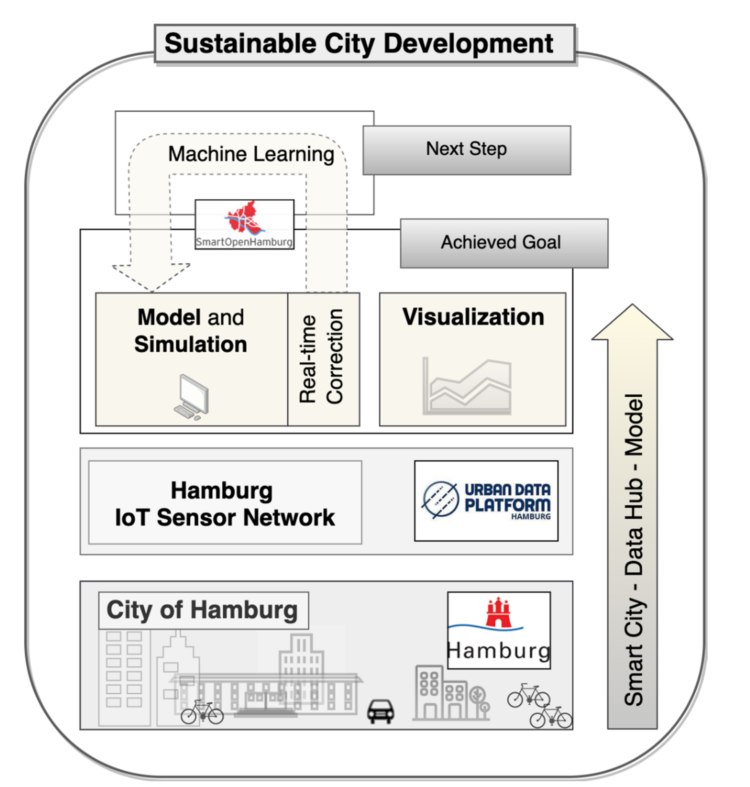
\includegraphics[width=0.75\textwidth]{lenfers-workflow}~\caption{Beispielworkflow, wie Daten aus den Sesnsoren und von der Stadt Hamburg in ein abstraktes Simulationsmodell eingebaut werden~\cite{Lenfers-MP-2021}}
    \label{fig:lenfers-workflow-sensors}
\end{figure}

Wie aus dem Workflow von~\ref{fig:lenfers-workflow-sensors} zu entnehmen ist, fokussiert sich der Kern der Arbeit aus dem Zusammenspiel von Datenfluss des Smart-City-Data-Hub und die Dateneinbindung von Fahrradverleihstationen in die SmartOpenHamburg-Komponente.
Echtzeitdaten werden bei ihrer Implementation von der ,,Smart City`` über ein zeitlichen Vektor-Layer in die Simulation konstant eingelesen und anhand ihrer Lebenszeit entsprechend simuliert\cite{Lenfers-MP-2021}.
Die Daten selbst werden dabei über eine URI von den externen Endpunkten abgefragt und mit zusätzlichen Argumenten auf die relevanten Daten reduziert~.
Mit diesem Datenstrom werden die derzeitigen Zustände der Fahrradverleihstationen abgefragt und in die Simulation eingebaut, wie viele Fahrräder derzeit aktuell aktiv genutzt werden und wie viele Agenten in der Simulation agieren\cite{Lenfers-MP-2021}.

Der Forschungsbeitrag von Lenfers und andere ist aber, wie bei der vorherigen, für diese Arbeit nur begrenzt relevant: Die statische Implementation von Fahrradverleihstationen ist relevant, da Verkehrsteilenhmer an den Stationen sich ein Fahrrad leihen können, doch ist dabei kein Echtzeitstrom vonnöten und passiert passiv nebenbei.

Dennoch bietet die Arbeit Anknüpfmöglichkeit, sollten relevanten Echtzeitdaten von der Stadt Hamburg zum Verkehr oder zu Lichtsignalanlagen über die nächste Zeit aufkommen und damit den Kern einer anderen Arbeit darstellen.


\textbf{Daniel Glake, Fabian Panse, Norbert Ritter, Thomas Clemen und Ulfia Lenfers:}
\textit{Incorporating Multi-Modal Travel Planning into an Agent-Based Model: A Case Study at the Train Station Kellinghusenstraße in Hamburg}

Der Forschungsartikel von Lenfers und andere aus dem Jahr 2021 erweitert ebenfalls das MARS-Framework und das SmartOpenHamburg-Projekt um nachhaltige Modalitäten wie die mietbaren Äquivalente zu Pkws und Fahrrädern oder das Zu-Fuß-Gehen.
Dabei untersuchen sie, wie effizient das Wechseln der Modalitäten in einem Beispielszenario ist und ob die Optimierungsstrategien hinsichtlich der Klimaneutralität, aus finanziellen Gründen oder persönlichen Präferenzen korrekt annähern~\cite{Lenfers-MMT-2021}.

Das Beispielszenario, welches sie zur Demonstrierung der implementierten Modalitäten verwenden, umfasst dabei die Bahnhofsstation Kelinghusenstraße in Hamburg, von der aus die Agenten mit den Modalitäten in einem Kreis-Bereich zu ihrem Ziel gelangen können.

\begin{figure}[h]
    \centering
    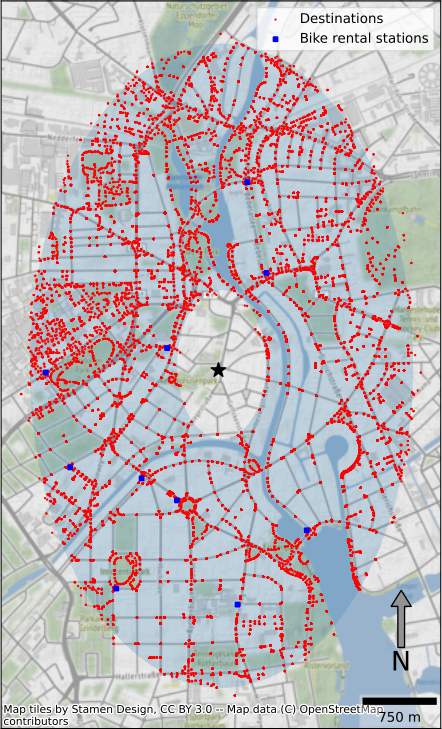
\includegraphics[width=0.75\textwidth]{lenfers-kelinghusen}~\caption{Karte der Fahrradverleihstationen, mit dem Simulationsbereich der Agenten hellblau hinterlegt, den Interessenspunkten rot markiert und Fahrradverleihstation als blaue Markierungen~\cite{Lenfers-MMT-2021}}
    \label{fig:lenfers-kelinghusen-area}
\end{figure}

Auf dem Weg zu ihrem Endziel innerhalb des simulierbaren Bereichs aus~\ref{fig:lenfers-kelinghusen-area} kommen manche Agenten durch angestrebtes Nutzen der Modalitäten erst zur nächsten Fahrrad- oder Pkwverleihstation, bevor sie ihre Reise zum Interessenspunkt fortsetzen können.
Dieses angestrebte Nutzen wird in den Eingabedaten durch zum Beispiel die Variablen ,,hasCar`` und ,,usesBikeAndRide`` versinnbildlicht, wie hoch die Wahrscheinlichkeit zum Nutzen oder Besitzen einer eigenen oder gemieteten Modalität ist~\cite{Lenfers-MMT-2021}.

Auf den implementierten Modalitäten und Verleihstationen aus der Forschungsarbeit von Lenfers und andere knüpft diese Arbeit hier an und untersucht nun mithilfe der Auswahl an Modalitäten eine mögliche Lichtsignalschaltung.
Damit bietet diese Arbeit eine sehr gute Grundlage, auf der nun aufgesetzt und das hier in dieser Arbeit beschriebenen Szenario aufgesetzt wird.
